\let\lesson\undefined
\newcommand{\lesson}{\phantomlesson{Bài 14.}}
\setcounter{section}{2}
\section{Trắc nghiệm}
\begin{enumerate}[label=\bfseries Câu \arabic*:, leftmargin=1.5cm]
	
	\item \mkstar{1}
	
	
	{Lực tác dụng vào vật làm cho vật quay quanh một trục có giá
		\begin{mcq}
			\item song song với trục quay.
			\item cắt trục quay.
			\item nằm trong mặt phẳng song song với trục quay.
			\item nằm trong mặt phẳng vuông góc với trục quay và không cắt trục quay.
		\end{mcq}
	}
	
	\hideall
	{	\textbf{Đáp án: D.}
		
		Lực tác dụng vào vật làm cho vật quay quanh một trục có giá nằm trong mặt phẳng vuông góc với trục quay và không cắt trục quay.
	}

\item \mkstar{1}\\
{Cánh tay đòn của lực bằng
	\begin{mcq}
		\item khoảng cách từ trục quay đến điểm đặt của lực.
		\item khoảng cách từ trục quay đến trọng tâm của vật.
		\item khoảng cách từ trục quay đến giá của lực.
		\item khoảng cách từ trọng tâm của vật đến giá của trục quay.
	\end{mcq}

}
\hideall{
\textbf{Đáp án C.}
}
	\item \mkstar{1}
	
	
	{Một ngẫu lực gồm có hai lực $\vec F_1$ và $\vec F_2$ có $F_1 = F_2 = F$ và có cánh tay đòn $d$. Momen ngẫu lực này là
		\begin{mcq}(2)
			\item $(F_1-F_2)d$.
			\item $2Fd$.
			\item $Fd$.
			\item Chưa xác định.
		\end{mcq}
	}
	
	\hideall
	{	\textbf{Đáp án: C.}
		
	}
	\item \mkstar{2}
	
	
	{Hai lực của ngẫu lực có độ lớn $F=\SI{20}{N}$, khoảng cách giữa hai giá của ngẫu lực là $d=\SI{30}{cm}$. Momen của ngẫu lực có độ lớn bằng
		\begin{mcq}(4)
			\item $\SI{0.6}{\newton\cdot\meter}$.
			\item $\SI{600}{\newton\cdot\meter}$.
			\item $\SI{6}{\newton\cdot\meter}$.
			\item $\SI{60}{\newton\cdot\meter}$.
		\end{mcq}
	}
	
	\hideall
	{	\textbf{Đáp án: C.}
		
		Momen của ngẫu lực:
		$$M=Fd = \SI{6}{\newton\cdot\meter}$$
	}

\item \mkstar{3}\\
{Một thanh đồng chất có chiều dài $L$, trọng lượng $\SI{200}{\newton}$, treo một vật có trọng lượng $\SI{450}{\newton}$ vào thanh như hình \ref{fig:23.5}. Các lực $\vec F_1$, $\vec F_2$ của thanh tác dụng lên hai điểm tựa có độ lớn lần lượt là
	\begin{center}
		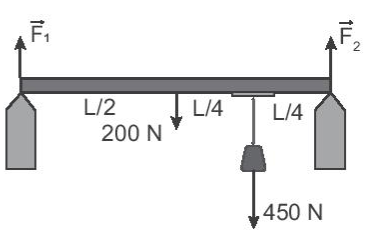
\includegraphics[width=0.4\linewidth]{../figs/VN10-2022-PH-TP023-P-5}
		\captionof{figure}{}
		\label{fig:23.5}
	\end{center}
\begin{mcq}(4)
	\item $\SI{212.5}{\newton}$; $\SI{437.5}{\newton}$.
	\item $\SI{325}{\newton}$; $\SI{325}{\newton}$.
	\item $\SI{437.5}{\newton}$; $\SI{212.5}{\newton}$.
	\item $\SI{487.5}{\newton}$; $\SI{162.5}{\newton}$.
\end{mcq}
}
\hideall{
\textbf{Đáp án A.}\\
Các lực thành phần theo phương $Oy$ cân bằng nhau:
\begin{equation}
	\label{eq:23.1}
	F_1+F_2-200-450=0
\end{equation}
Áp dụng quy tắc moment lực đối với trục quay tại A:
\begin{equation}
	\label{eq:23.2}
	\dfrac{L}{2}\cdot 200+\dfrac{3L}{4}\cdot 450=LF_2
\end{equation}
Từ (\ref{eq:23.1}) và (\ref{eq:23.2}), suy ra $F_1=\SI{212.5}{\newton}$, $F_2=\SI{437.5}{\newton}$.
}

\item\mkstar{3}\\
{Một đường ống đồng chất có trọng lượng $\SI{100}{\newton}$, chiều dài $L$, tựa trên điểm tựa như hình \ref{fig:23.3}. Khoảng cách $x$ và phản lực $F_R$ của điểm tựa tác dụng lên đường ống là
	\begin{center}
		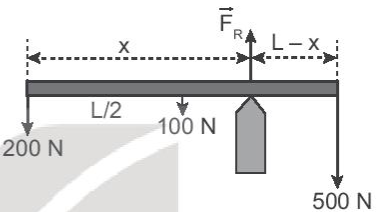
\includegraphics[width=0.4\linewidth]{../figs/VN10-2022-PH-TP023-P-3}
		\captionof{figure}{}
		\label{fig:23.3}
	\end{center}
\begin{mcq}(2)
	\item $x=0,69L$; $F_R=\SI{800}{\newton}$.
	\item $x=0,69L$; $F_R=\SI{400}{\newton}$.
	\item $x=0,6L$; $F_R=\SI{552}{\newton}$.
	\item $x=0,6L$; $F_R=\SI{248}{\newton}$.
\end{mcq}

}
\hideall{
\textbf{Đáp án A.}\\
Áp dụng quy tắc moment lực đối với trục quay tại A.
\begin{center}
	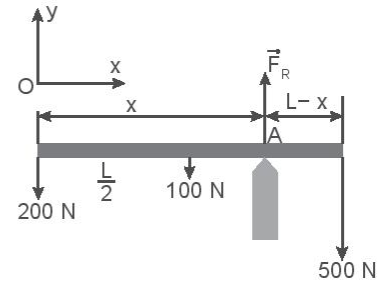
\includegraphics[width=0.4\linewidth]{../figs/VN10-2022-PH-TP023-P-4}
\end{center}
$$x\cdot 200+\left(x-\dfrac{L}{2}\right)\cdot100=\left(L-x\right)\cdot500$$
$$\Rightarrow x=0,69L$$
Các lực thành phần theo phương $Oy$:
$$F_R-200-100-500=0\Rightarrow F_R=\SI{800}{\newton}.$$
}

\item \mkstar{3}\\
{Một thanh chắn đường dài $\SI{7.8}{\meter}$, có trọng lượng $\SI{2100}{\newton}$ và có trọng tâm
ở cách đầu bên trái $\SI{1.2}{\meter}$. Thanh có thể quay quanh một trục nằm ngang ở cách đầu bên trái $\SI{1.5}{\meter}$. Hỏi phải tác dụng vào đầu bên phải một lực tối thiểu bằng bao nhiêu để thanh ấy nằm ngang?
\begin{mcq}(4)
	\item $\SI{100}{\newton}$.
	\item $\SI{200}{\newton}$.
	\item $\SI{300}{\newton}$.
	\item $\SI{400}{\newton}$.
\end{mcq}

}
\hideall{
\textbf{Đáp án A.}\\
\begin{center}
	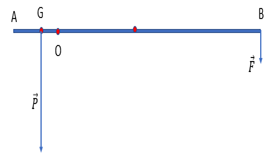
\includegraphics[width=0.4\linewidth]{../figs/VN10-2022-PH-TP023-P-1}
\end{center}
Áp dụng quy tắc moment cho trục quay qua O:
$$P\cdot OG=F\cdot OB$$
$$\Rightarrow F=\dfrac{P\cdot OG}{OB}=\dfrac{\left(\SI{2100}{\newton}\right)\cdot\left(\SI{0.3}{\meter}\right)}{\SI{7.8}{\meter}-\SI{1.5}{\meter}}=\SI{100}{\newton}.$$
}
	
	\item \mkstar{3}\\
	{Một tấm ván nặng $\SI{270}{\newton}$ được bắc qua một con mương. Trọng tâm của tấm ván cách điểm tựa trái $\SI{0.8}{\meter}$ và cách điểm tựa phải là $\SI{1.6}{\meter}$. Hỏi lực mà tấm ván tác dụng lên điểm tựa bên trái là bao nhiêu?
		\begin{mcq}(4)
			\item $\SI{180}{\newton}$.
			\item $\SI{90}{\newton}$.
			\item $\SI{160}{\newton}$.
			\item $\SI{80}{\newton}$.
		\end{mcq}
}
\hideall{
\textbf{Đáp án A.}\\
\begin{center}
	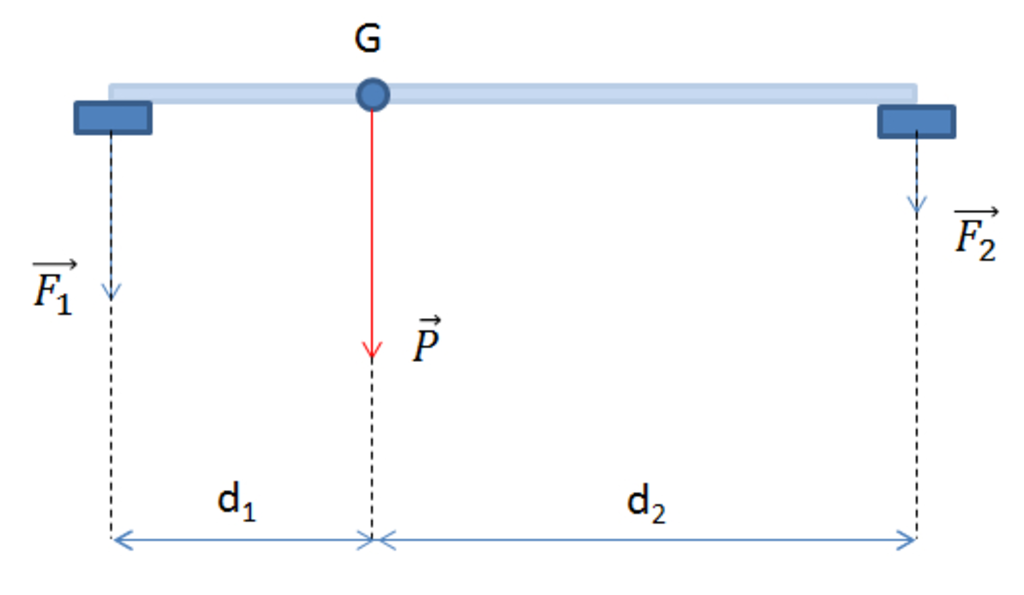
\includegraphics[width=0.4\linewidth]{../figs/VN10-2022-PH-TP023-P-2}
\end{center}
Áp dụng quy tắc moment cho trục quay qua điểm tựa phải:
$$P\cdot d_2=F'_1\cdot\left(d_1+d_2\right)$$
với $\vec F'_1=-\vec F_1$ là lực do điểm tựa trái tác dụng lên ván.
$$\Rightarrow F'_1=\dfrac{P\cdot d_2}{d_1+d_2}=\SI{180}{\newton}$$
Lực do ván tác dụng lên điểm tựa trái:
$$F_1=F'_1=\SI{180}{\newton}.$$
}
	
	\item \mkstar{3}
	
	
	{Một thanh nhẹ gắn vào sàn tại B như hình vẽ.
		\begin{center}
			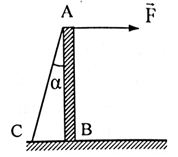
\includegraphics[scale=1]{../figs/VN10-2021-PH-TP021-6.png}
		\end{center}
		Tác dụng lên đầu A lực kéo $F=\SI{100}{N}$ theo phương ngang. Thanh được giữ cân bằng nhờ dây AC. Lực căng của dây có giá trị là bao nhiêu? Biết $\alpha = 30^\circ$.
		\begin{mcq}(4)
			\item $\SI{250}{N}$.
			\item $\SI{150}{N}$.
			\item $\SI{100}{N}$.
			\item $\SI{200}{N}$.
		\end{mcq}
	}
	
	\hideall
	{	\textbf{Đáp án: D.}	
		
		Chọn trục quay tại B. Áp dụng quy tắc momen lực:
		$$F \cdot \text{AB} = T \cdot \text{AB} \cdot \sin \alpha \Rightarrow T = \dfrac{F}{\sin \alpha} = \SI{200}{N}$$
	}
	
	
	
	\item \mkstar{4}
	
	
	{Bán cầu đồng chất khối lượng $\SI{100}{g}$. Trên mép bán cầu đặt một vật nhỏ khối lượng $\SI{7.5}{g}$. Hỏi mặt phẳng của bán cầu sẽ nghiêng góc $\alpha$ bao nhiêu khi nó cân bằng? Biết rằng trọng tâm bán cầu cách mặt phẳng của bán cầu một đoạn $3R/8$ (với $R$ là bán kính của bán cầu).
		\begin{center}
			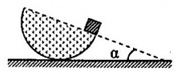
\includegraphics[scale=1]{../figs/VN10-2021-PH-TP021-7.png}
		\end{center}
		\begin{mcq}(4)
			\item $11,31^\circ$.
			\item $15^\circ$.
			\item $20^\circ$.
			\item $12^\circ$.
		\end{mcq}
	}
	
	\hideall
	{	\textbf{Đáp án: A.}
		
		\begin{center}
			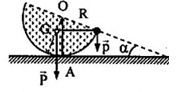
\includegraphics[scale=1]{../figs/VN10-2021-PH-TP021-8.png}
		\end{center}
		
		Các lực tác dụng lên bán cầu: trọng lực $\vec P$ của bán cầu, trọng lực $\vec p$ của vật nhỏ, phản lực $\vec Q$ tại điểm tiếp xúc A.
		
		Áp dụng quy tắc momen lực với trục quay qua O:
		$$P \cdot \text{OG} \cdot \sin \alpha = p \cdot R \cdot \cos \alpha \Rightarrow \tan \alpha = \dfrac{8m}{3M} \Rightarrow \alpha = 11,31^\circ$$
	}
	
	
\end{enumerate}



\ANSMCQ
{
	\begin{center}
		\begin{tabular}{|m{2.8em}|m{2.8em}|m{2.8em}|m{2.8em}|m{2.8em}|m{2.8em}|m{2.8em}|m{2.8em}|m{2.8em}|m{2.8em}|}
			\hline
			1.D  & 2.C  & 3.C & 4.C & 5.A  & 6.A & 7.A & 8.A & 9.D & 10.A  \\
			\hline
			
		\end{tabular}
	\end{center}
}
\section{Tự luận}
\begin{enumerate}[label=\bfseries Câu \arabic*:, leftmargin=1.5cm]
	\item \mkstar{1}
	
	{
		Momen lực đối với một trục quay là gì? Phát biểu điều kiện cân bằng của một vật có trục quay cố định (hay quy tắc momen lực).
	}
	
	\hideall{
		Momen lực đối với một trục quay là đại lượng đặc trưng cho tác dụng làm quay của lực và được đo bằng tích của lực với cánh tay đòn của nó.
		$$M=Fd,$$
		trong đó:
		\begin{itemize}
			\item $F$ là lực tác dụng $(\SI{}{N})$;
			\item $d$ là cánh tay đòn (là khoảng cách từ giá của lực đến trục quay) $\SI{}{m}$.
		\end{itemize}
		
		Muốn một vật có trục quay cố định nằm cân bằng thì tổng các momen lực có xu hướng làm cho vật quay theo chiều kim đồng hồ phải bằng tổng các momen lực có xu hướng làm cho vật quay ngược chiều kim đồng hồ.
	}
	
	\item \mkstar{2}
	
	
	{Hãy giải thích hoạt động của chiếc cân (hình vẽ).
		\begin{center}
			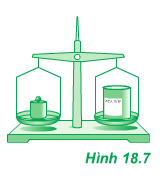
\includegraphics[scale=1]{../figs/VN10-2021-PH-TP021-5.png}
		\end{center}
	}
	
	\hideall
	{
		Khi cân nằm cân bằng (kim chỉ thẳng đứng), theo quy tắc momen lực, ta có:
		$$P_\text{vật} d_1 = P_\text{cân} d_2$$
		
		Vì $d_1=d_2$ nên khi đó $P_\text{vật} = P_\text{cân}$. Suy ra khối lượng vật cần đo bằng khối lượng của quả cân.
		
		Cân hoạt động theo quy tắc momen lực.
	}
	
	
	\item \mkstar{2}\\
	{Một cái thước $AB=\SI{1.2}{\meter}$ đặt trên mặt bàn nhẵn nằm ngang, có trục quay O cách đầu A một khoảng $\SI{80}{\centi\meter}$. Một lực $F_1=\SI{5}{\newton}$ tác dụng lên đầu A theo phương vuông góc với thước và lực thứ hai tác dụng lên đầu B của thước theo phương vuông góc với thước. Các lực đều nằm trên mặt phẳng nằm ngang. Nếu thước không chuyển động thì lực tác dụng vào đầu B của thước có hướng và độ lớn như thế nào?
		\begin{center}
			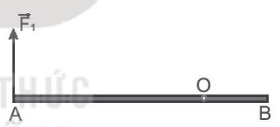
\includegraphics[width=0.35\linewidth]{../figs/VN10-2022-PH-TP023-P-8}
		\end{center}
	
}
\hideall{
$\vec F_2$ cùng hướng với $\vec F_1$.\\
Áp dụng quy tắc moment cho trục quay qua O:
$$F_1\cdot OA=F_2\cdot OB\Rightarrow F_2=\dfrac{F_1\cdot OA}{OB}=\dfrac{\left(\SI{5}{\newton}\right)\cdot\left(\SI{0.8}{\meter}\right)}{\SI{0.4}{\meter}}=\SI{10}{\newton}.$$

}

\item \mkstar{2}\\
{Một thanh kim loại đồng chất AB dài $\SI{2}{\meter}$ có tiết diện đều và khối lượng của thanh là $\SI{2}{\kilo\gram}$. Người ta treo vào đầu A của thanh một vật có khối lượng $\SI{5}{\kilogram}$, đầu B một vật có khối lượng $\SI{1}{\kilogram}$. Hỏi phải đặt một giá đỡ tại điểm O cách đầu A một khoảng là bao nhiêu để thanh cân bằng?
}
\hideall{
\begin{center}
	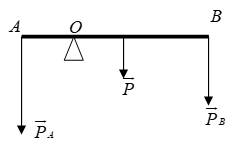
\includegraphics[width=0.3\linewidth]{../figs/VN10-2022-PH-TP023-P-9}
\end{center}
Gọi O là vị trí điểm tựa.\\
Áp dụng quy tắc moment cho trục quay qua O:
\begin{eqnarray*}
	&&P_\text{A}\cdot OA=P\cdot OG+P_\text{B}\cdot OB\\
	&\Leftrightarrow &P_\text{A}\cdot OA=P\cdot\left(\dfrac{AB}{2}-OA\right)+P_\text{B}\cdot\left(AB-OA\right)\\
	&\Leftrightarrow &50\cdot OA=20\cdot\left(1-OA\right)+10\cdot\left(2-OA\right)\\
	&\Rightarrow &OA=\SI{0.5}{\meter}.
\end{eqnarray*}
}

\item\mkstar{3}\\
{Một thanh sắt dài, đồng chất, tiết diện đều, được đặt trên bàn sao cho $\frac{1}{4}$ chiều dài của nó nhô ra khỏi bàn. Tại đầu nhô ra, người ta đặt một lực $\vec F$ thẳng đứng hướng xuống dưới. Khi lực đạt tới giá trị $\SI{40}{\newton}$ thì đầu kia của thanh sắt bắt đầu bênh lên. Hỏi trọng lượng của thanh sắt bằng bao nhiêu?
	\begin{center}
		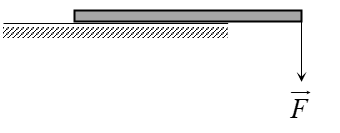
\includegraphics[width=0.4\linewidth]{../figs/VN10-2022-PH-TP023-P-10}
	\end{center}

}
\hideall{
Áp dụng quy tắc moment với điểm tựa tại cạnh bàn:
\begin{eqnarray*}
	&&P\cdot\left(\dfrac{L}{2}-\dfrac{L}{4}\right)=F\cdot\dfrac{L}{4}\\
	&\Rightarrow& F=P=\SI{40}{\newton}.
\end{eqnarray*}
}

\item \mkstar{3}\\
{Một thanh có độ dài $L$, trọng lượng $\SI{10}{\newton}$, được treo nằm ngang vào tường như hình \ref{fig:23.6}. Một vật có trọng lượng $\SI{20}{\newton}$ treo ở đầu thanh. Dây treo hợp với thanh một góc $\alpha=\SI{30}{\degree}$. Xác định lực căng dây treo.
	\begin{center}
		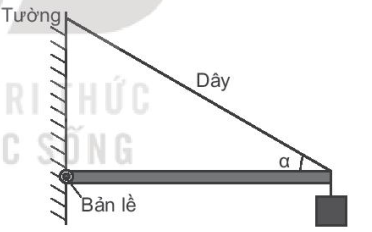
\includegraphics[width=0.4\linewidth]{../figs/VN10-2022-PH-TP023-P-6}
		\captionof{figure}{}
		\label{fig:23.6}
	\end{center}

}
\hideall{
Áp dụng quy tắc moment đối với trục quay qua O:
\begin{center}
	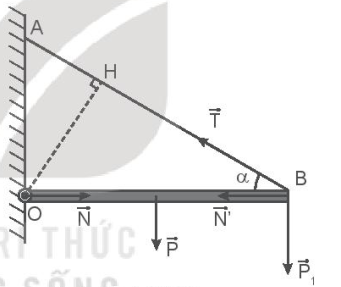
\includegraphics[width=0.35\linewidth]{../figs/VN10-2022-PH-TP023-P-7}
\end{center}
$$0\cdot N+OH\cdot T=\dfrac{L}{2}\cdot P+L\cdot P_1$$
$$\Leftrightarrow T\cdot L\sin\alpha=\dfrac{L}{2}\cdot P+L\cdot P_1$$
$$\Rightarrow T=\dfrac{\dfrac{P}{2}+P_1}{\sin\alpha}=\dfrac{\SI{5}{\newton}+\SI{20}{\newton}}{\sin\SI{30}{\degree}}=\SI{50}{\newton}.$$
}

	\item \mkstar{4}
	
	
	{Một vật rắn phẳng, mỏng, có dạng là một hình vuông ABCD, mỗi cạnh là $a=\SI{10}{cm}$. Người ta tác dụng một ngẫu lực nằm trong mặt phẳng của hình vuông. Biết các lực vuông góc với đường chéo AD có độ lớn $\SI{10}{N}$ và đặt vào hai đỉnh của A và D. Tính momen của ngẫu lực.
	}
	
	\hideall
	{Ta có đường chéo của hình vuông:
		$$d=\sqrt{a^2 + a^2} = \SI{14.14}{cm} = \SI{0.14}{m}$$
		
		Momen ngẫu lực:
		$$M=Fd = \SI{1.41}{Nm}$$
	}
\end{enumerate}